\chapter{Resultados}
\label{ch:Resultados}
\section{Processo de AM}
Esta seção descreve a realização do processo de AM, deste a coleta até a apresentação dos dados.
\subsection{Coleta}
A coleta dos dados foi realizada pelos pesquisadores Jorge Luiz (Engenheiro Eletricista) e Bruna da Silva (Fisioterapeuta), utilizanda o protocolo descrito no Apendice \ref{apendicetae}, o qual descreve detalhadamente todo o processo de coleta dos dados.

Os dados utilizados para a classificação, se refem a \textbf{Coleta 1 - Tremor de Repouso}, uma vez que esta apresentou os melhores resultados na classificação, já que as outras três coletas apresentavam um alto ruído que acabaram comprometendo os dados. A seguir um pequeno resumo sobre esta coleta.

Foram realizadas três coletas por colaborador, com duração de cinco segundos cada, a disposição dos eletrodos encontra-se no Apendice \ref{apendicetae}. Os dados do sinal foram aramazenadas através da utilização de 4 canais, sendo eles:
\begin{enumerate}
    \item \textbf{CH1}: Extensor radial do longo do carpo direito;
    \item \textbf{CH2}: Flexor superficial dos dedos direito;
    \item \textbf{CH3}: Extensor radial do longo do carpo esquerdo;
    \item \textbf{CH4}: Flexor superficial dos dedos esquerdo.
\end{enumerate}

Estes dados coletados em sEMG em cada canal, foram cedidos no formato \textit{edf}.

\subsection{Processamento dos dados}
Com os dados brutos iniciou-se a etapa de pré-processamento dos dados. Inicialmente utilizou-se como tecnica para a filtragem dos dados a Transformada rápida de Fourier (FFT), onde realizou-se testes nos quatro canais disponiveis, realizando um comparativo da acuracia com e sem a FFT, além de um comparativo sobre a acuracia entre os canais. 

Com relação aos dados obtidos em cada canal, como pode ser obsrvado na figura \ref{fcomparativo}, utilizando a fft obteve-se um bom resultado nos canais \textbf{CH1} com uma precisão de 78 e um resultado razoavel no \textbf{CH3} com precisão em 69.

Realizou-se também a aplicação de filtros de frequência, passa-banda, passa-baixa e passa-alta. Porém estes filtros diminuiram a acuracia obtida, como observado na figura \ref{comesemfiltro}, que exemplifica a matriz de confusão referente ao \textbf{CH1}, assim como normalizou-se os dados em diferentes escalas e do mesmo modo a acuracia caiu.

% \begin{figure}[!htb]
% 	\centering
% 	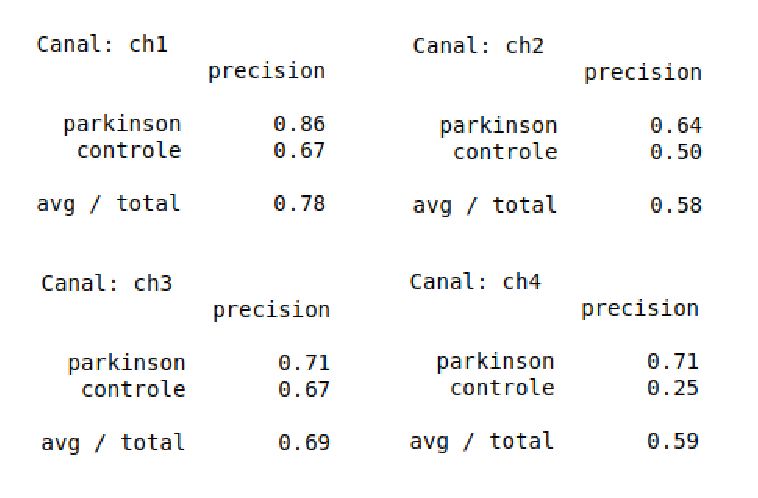
\includegraphics[width=1.1\textwidth]{figuras/fcomparativo.eps}
% 	\caption{Comparativo entre os canais, com a fft.}
% 	\label{fcomparativo}
% \end{figure}

\begin{figure}[!htb]
	\centering
	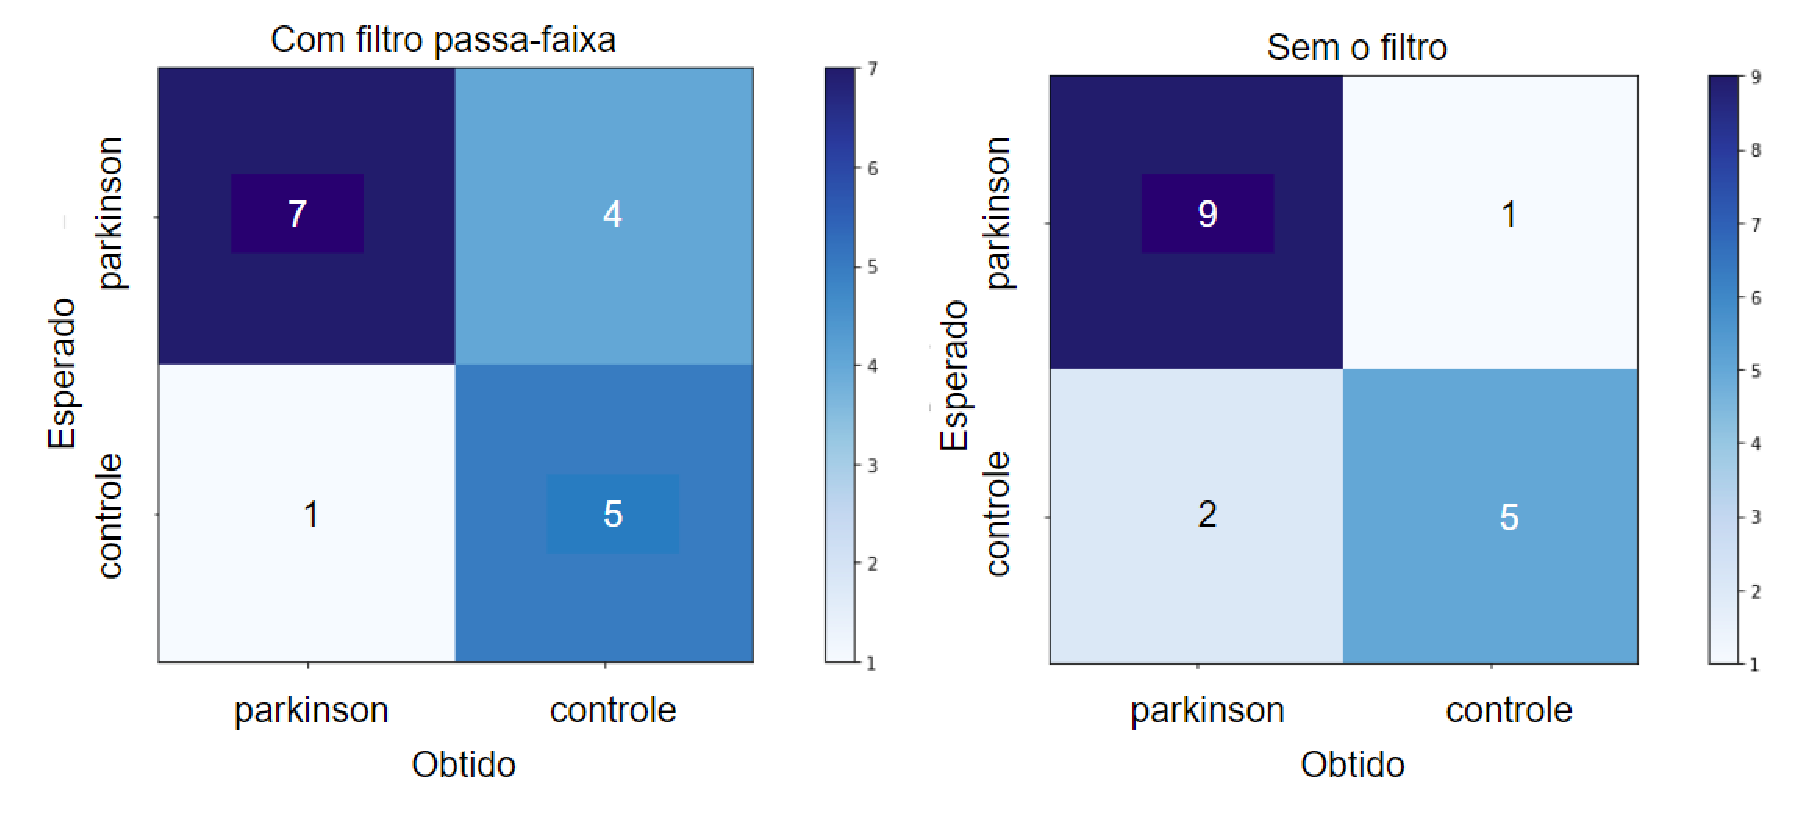
\includegraphics[width=1.1\textwidth]{figuras/comesemfiltro.eps}
	\caption{Matriz de confusão com e sem filtro do \textbf{Ch1}.}
	\label{comesemfiltro}
\end{figure}

Também realizou-se a classificação utilizando todos os canais ao mesmo tempo, porém o resultado foi insatisfatorio.

Outra técnica de selecão de feature utilizada foi a PCA ou Análise de componentes principais, com a utilização desta tecnica obteve-se uma leve melhora na acuracia, como pode ser observado na figura \ref{pcavalidator}, a qual utilizou-se o \textit{k-fold cross-validator} para verificar a precisão real do modelo.

Como pode ser observado na figura \ref{pcavalidator}, com o auxilio do k-fold, pode-se inferir que o Random Forest possui uma precisão superior ao SVM, além de que o PCA aumenta a acuracia consideravelmente do modelo.

\begin{figure}[!htb]
	\centering
	\includegraphics[width=1.1\textwidth]{figuras/pcavalidator.eps}
	\caption{Matriz de confusão com e sem filtro do canal 1.}
	\label{pcavalidator}
\end{figure}

Finalizando a etapa de pré-processamento dos dados, concluiu-se que a utilização da FFT com o PCA mostrou-se a melhor combinação para obtermos os melhores resultados, com o \textit{Random Forest} levemente superior ao SVM e o KNN, com as respectivas precisões.

\subsection{Apresentar dos dados}

\section{Solução de software}
Como descrito no documento de Visão {citar anexo visão} e no documento de Arquitetura { citar documento de Arquitetura}.
\subsection{Arquitetura}

\subsection{Visão}
O documento de Visão encontra-se no anexo \ref{adocvisao} na página \pageref{adocvisao}.

\subsection{Produto}
O documento de Arquitetura

% \section{Resultados parciais}
% \section{Abstrair o problema no contexto}
% O contexto geral do trabalho é projetar e construir um sistema AM para auxiliar no diagnóstico da doença de Parkinson, utilizando sinais obtidos por dispositivos sEMG, e o problema principal gira em torno de como esse sistema será desenvolvido. Por se tratar da construção de um software, isso necessita de um planejamento prévio de como será feita essa construção, levando em consideração um conjunto de variáveis para tomada de decisões. Neste trabalho o sistema a ser desenvolvido se trata de um sistema AM, que requer uma maior atenção sobre algumas variáveis, como quantidade de recursos e tipos de dados obtidos, sendo que essas variáveis servem como indicadores para auxiliar a decisão de qual algoritmo utilizar para se encontrar a melhor solução possível para esse problema.

% \section{Prova de conceito}
% Para verificar a viabilidade do projeto, além de buscar entender o fu ncionamento da biblioteca \textit{scikit-learn}. Realizou-se uma prova de conceito, desenvolvendo um algoritmo utilizando o SVM, para predizer os dados relacionados a uma porta lógica XOR. Foram utilizados também o \textit{numpy} para as manipulações matemáticas e o \textit{matplotlib} para plotar o gráfico. Para o teste utilizou-se 500 amostras. Sendo que estas foram separadas em 75\% em dados de treino e os 25\% restantes em dados de teste. Ou seja, 125 dados de treino e 375 dados de teste, não utilizou-se dados de validação.

% Como observado na Figura \ref{svmxor} na página \pageref{svmxor}, o svm conseguiu separar corretamente a maioria dos dados, sendo que, na imagem as bolas laranjas equivalem ao valor esperado “1”, e as bolas azuis equivalem ao valor esperado “0”. Já os contornos equivalem ao valor atingido pelo SVM, ou seja, as bolas dentro da área roxa foram preditas como “0” e  a bolas na área laranjada foram preditas como “1”. Também é possível observar nessa imagem os hiperplanos de separação.

% Utilizou-se também para verificar a precisão do modelo, a matriz de confusão, como pode ser observado na Figura \ref{mcxor} na página \pageref{mcxor}, e na Figura \ref{mcxornormalizada} na página \pageref{mcxornormalizada}, a qual mostra a matriz de confusão normalizada com a porcentagem de dados.

% Outra ferramenta utilizada foi a \textit{Classification report} Figura \ref{class_report} na página \pageref{class_report}, que descreve separadamente a taxa de precisão, além de outros conceitos da estatística.

% \begin{figure}[!htb]
% 	\centering
% 	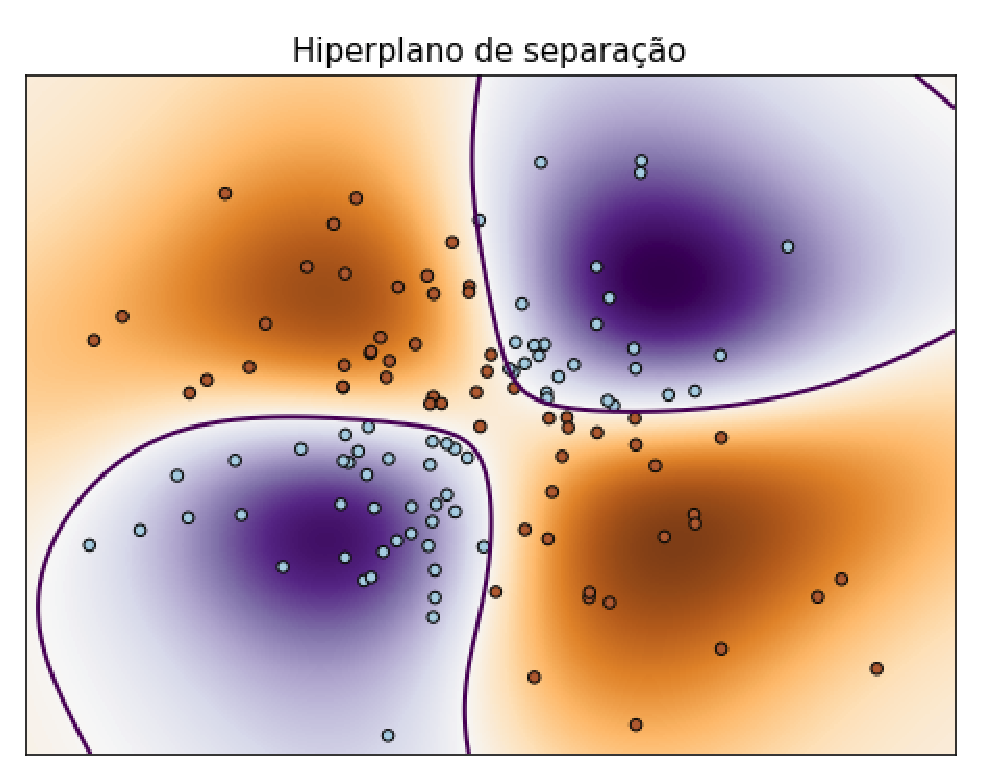
\includegraphics[width=0.8\textwidth]{figuras/xor.eps}
% 	\caption{Hiperplano de separação do SVM na porta XOR.}
% 	\label{svmxor}
% \end{figure}

% \begin{figure}[!htb]
% 	\centering
% 	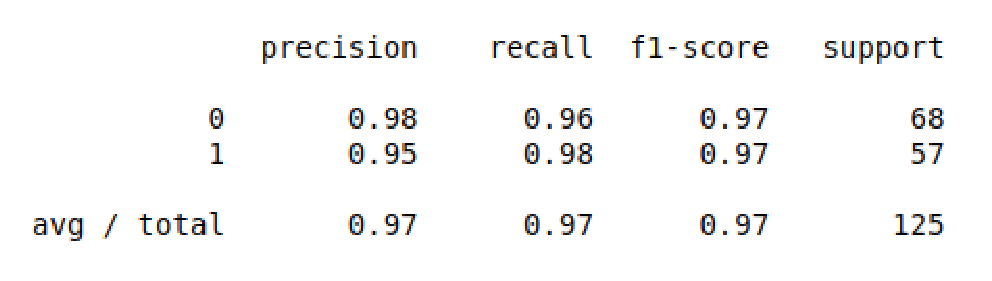
\includegraphics[width=0.8\textwidth]{figuras/class_report.eps}
% 	\caption{\textit{Classification report} da porta XOR.}
% 	\label{class_report}
% \end{figure}

% \begin{figure}[!htb]
% 	\centering
% 	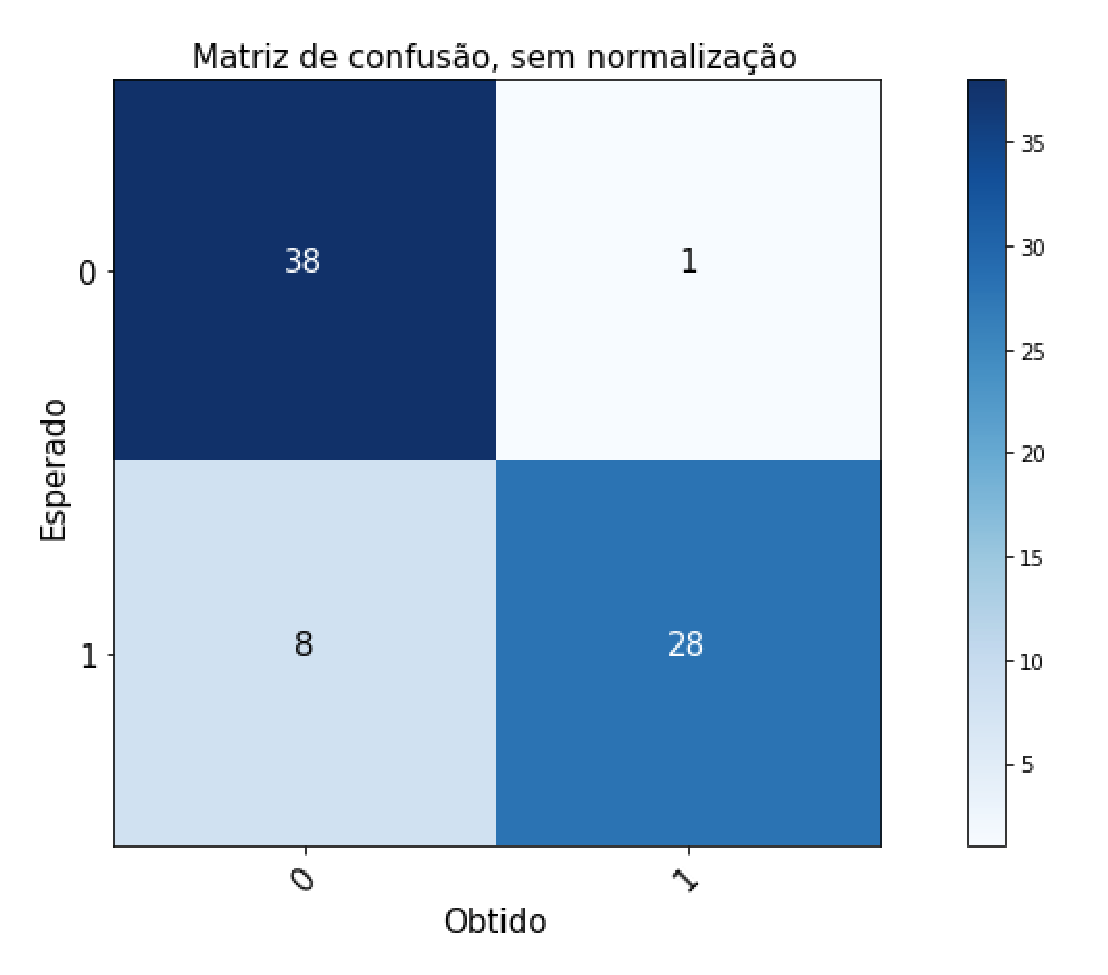
\includegraphics[width=0.8\textwidth]{figuras/mcxor.eps}
% 	\caption{Matriz de confusão da porta XOR.}
% 	\label{mcxor}
% \end{figure}

% \begin{figure}[!htb]
% 	\centering
% 	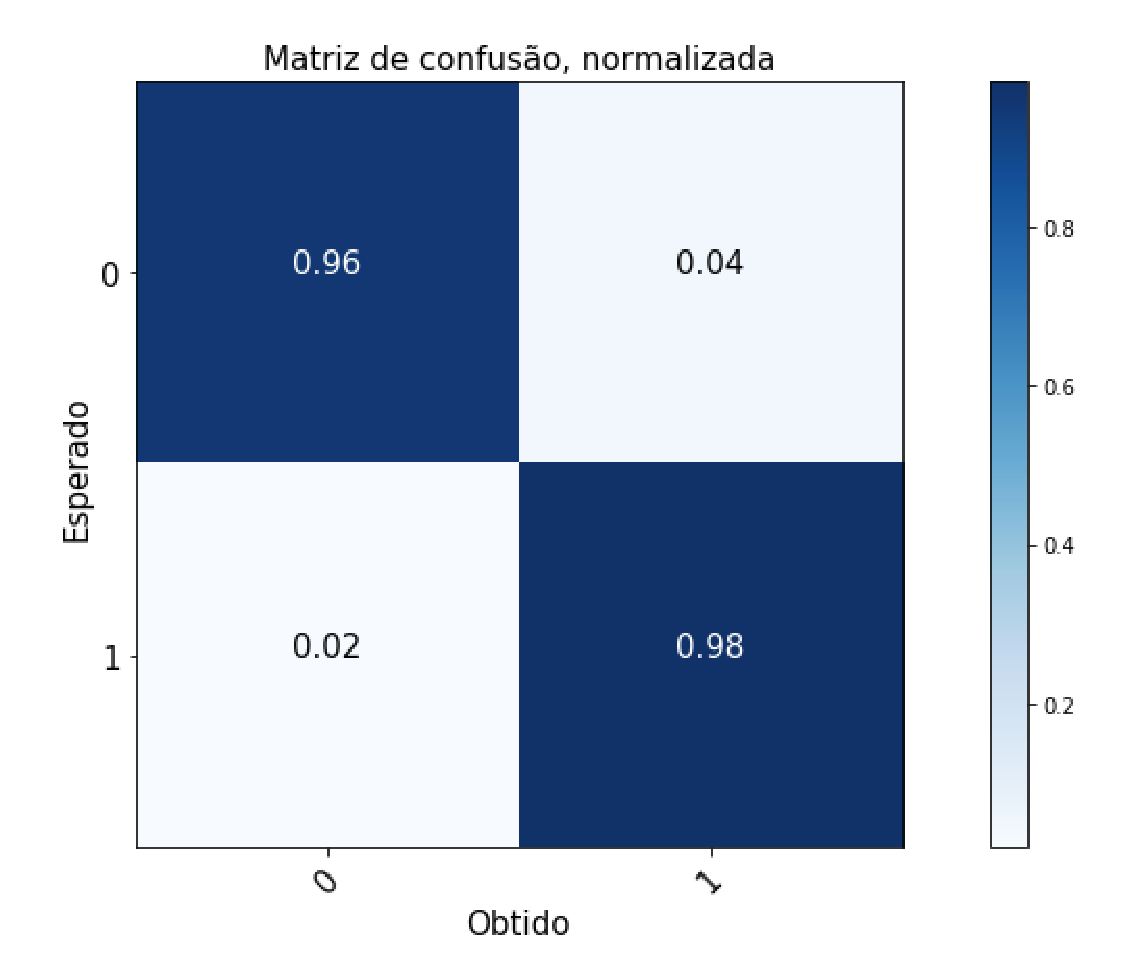
\includegraphics[width=0.8\textwidth]{figuras/mcxornormalizada.eps}
% 	\caption{Matriz de confusão normalizada da porta XOR.}
% 	\label{mcxornormalizada}
% \end{figure}
